\documentclass[fontset=windows,a4paper,12pt]{ctexart}
\usepackage{graphicx}
\usepackage{subfigure}
\usepackage{graphics}
\usepackage{overcite}
\usepackage{CJK}

\pagestyle{plain}
\usepackage{bm}
\usepackage{amsmath}
\usepackage{multirow}

\evensidemargin 3mm \oddsidemargin 3mm
\textwidth 154mm \textheight 225mm

\begin{document}

\begin{titlepage} \begin{center} % Upper part of the page 
  \textsc{\LARGE 2016数学建模校赛}\\
  [1.5cm] \textsc{\Large 题目\quad B}\\
  [0.5cm]\ \\
  [0.4cm] { \huge \bfseries 印制电路板焊锡}\\[0.4cm]\ \\[1.5cm]\ \\[1.4cm]\ 
  \large {学\quad\quad 校:} 
  \begin{minipage}[t]{0.4\textwidth}
    \centering
    \uline{\hspace{3em}山西大学\hfill} \makebox[0.46em]{}\par
  \end{minipage}
  \\[0.6cm]
  \large {队\quad\quad 员:} 
  \begin{minipage}[t]{0.4\textwidth} 
    \uline{\hspace{3em}李恩宾 \hfill} \makebox[0.46em]{}\par
    \uline{\hspace{3em}张红若 \hfill} \makebox[0.46em]{}\par
    \uline{\hspace{3em}张彪\quad \hfill} \makebox[0.46em]{}\par
  \end{minipage}
  \\[0.6cm]
  \large {指导教师:} 
  \begin{minipage}[t]{0.4\textwidth}
    \centering
    \uline{\hspace{3em}李顺勇 \hfill} \makebox[0.46em]{}\par
  \end{minipage}
  \vfill % Bottom of the page 
  {\large \today} \end{center} \end{titlepage}
  \begin{center}
    \zihao{3}{\heiti 印制电路板焊锡}
  \end{center}
  \linespread{1.2}
  \begin{center}
    \zihao{4}{\heiti 摘\ \ \ \ 要}
  \end{center}
  \zihao{4}{\songti 
    针对电路板焊锡过程中点胶机的涂锡膏顺序问题,本文将电路板中所有的位点抽
    象为图中的顶点,将位点间的连边抽象成顶点间的连边,位点间的距离抽象为边
    上的权值,构建赋权完全图。通过遗传算法和贪婪算法,求解赋权完全图中的最
    小哈密尔顿圈,即求得最优焊锡顺序和相应的路径长度。\cite{楼建华2003数学建模与数学实验}
  }
  \\
  关键词:\ 遗传算法\ 旅行商问题\ 贪婪算法\ 蚁群算法

  \newpage
  \tableofcontents
  \newpage
  \section{问题的提出}
    焊锡是印制电路板生产过程中的一步后续处理,目的是把贴片元件焊接到电路板表面。
    人们使用一台装有锡膏点胶机的数控(计算机数字控制,简称CNC)机械,将锡膏涂布
    于电路板表面的特定位置。现有一个电路板,大小为$300mm\times180mm$,共有280
    个位点需要点涂锡膏。

    问题一:求解点胶机从1号位点开始对这280个位点进行焊锡,最后回到1号位点的最优
    焊锡顺序,并给出相应路径长。

    问题二:不预先设定起点和终点,求解对1万张这种类型的电路板进行焊锡的最优顺序
    ,并给出相应路径长,这里假设每张电路板安装点胶机所需时间和所处位置都是相同的。
  \section{模型假设}
    \begin{enumerate}
      \item 假设点胶机的初始位置位于电路板起始位点的正上方;
      \item 假设电路板上的位点大小均一致;
    \end{enumerate}
  \section{符号说明}
  \section{模型的建立}
    \subsection{问题分析}
      通过对电路板焊锡问题的分析,我们将焊锡过程转化为赋权完全图中求最小哈密尔顿
      圈问题,即TSP旅行售货员问题。TSP问题是典型的NP-hard问题,不存在多项式时间
      算法求其最优解。我们通过建立贪婪算法和遗传算法,对电路板上的位点进行遍历
      ,最终回到起点,得到最优焊锡顺序,求得相应的路径长。
      
      将问题看做定义在图$G=(V,E)$上的TSP问题,其中$V={1,2,\dots,n}$,$E=(i,j),i,j\in V$
      图中节点之间的距离矩阵为
      
      \begin{equation}
      D=\left[
      \begin{array}{cccc}
      	0 & d_{1,2} & \dots & d_{1,n}\\
      	d_{2,1} & 0 & \dots & d_{2,n}\\
      	\dots & \dots & 0 & \dots \\
      	d_{n,1} & \dots & \dots & 0 \\
      \end{array}
      \right]
      \end{equation}
    \subsection{问题一}
	   \subsubsection{蚁群算法}
		   蚁群算法是通过模拟蚂蚁群体觅食行径而提出来的一种模拟进化算法\cite{士勇2004蚁群算法及其应用}。
	       蚁群算法结果如图\ref{fig:anti},总长度为$2946.44724482$
    	   \begin{figure}[htbp]
    	   	 \centering
    	   	 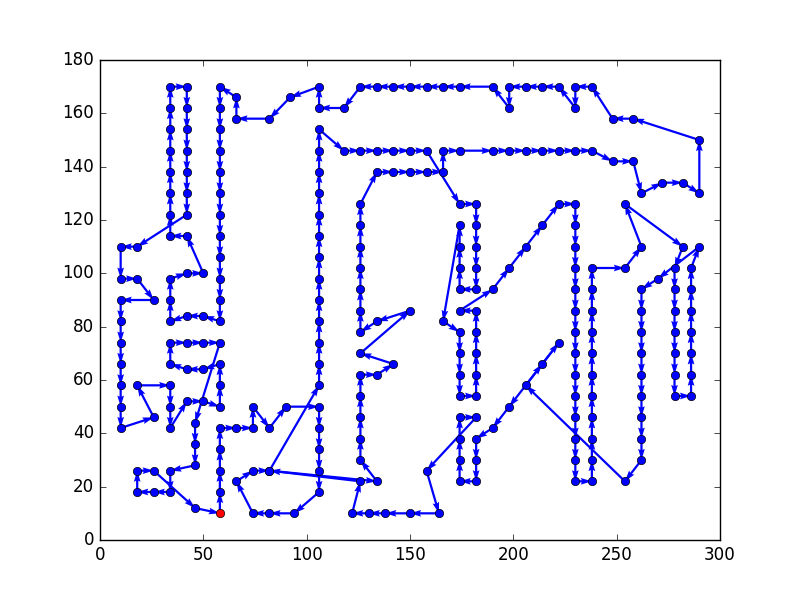
\includegraphics[width=10cm]{pic/anti_result.png}
    	   	 \caption{改进贪婪算法得到的结果}
    	   	 \label{fig:anti}
    	   \end{figure}
    	 
      \subsubsection{遗传算法}
      
      遗传算法是模仿生物进化过程的一种算法,它以自然选择和遗传学中的复制、变异和交叉等自然规律为理
      论依据。利用GA算法求解问题,首先需要将模型的解以适当的方式进行编码,并根据模型的目标建立
      个体适应度函数,然后随机生成初始种群(即一组初始的可行解),再重复对种群进行选择、交
      叉、变异等遗传操作直到种群成熟,停止优化\cite{赵静2008数学建模与数学实验}。
      对于NP困难问题智能算法是有效的的选择,我们选用遗传算法对问题一进行建模求解,并且根据实际题目的要求对遗传算法进行微调。
        
      %\subsubsection{变异与交叉算子}
      在一般的遗传算法中,种群个体j结构如图\ref{fig:life}所示,变异算子是指让种
      群中某个个体的某些基因突变的算子,
		\begin{figure}[htbp]
			\centering
			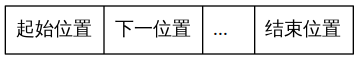
\includegraphics[width=5cm]{pic/life_struct.png}
			\caption{算法中的个体}
			\label{fig:life}
		\end{figure}
        由于本题限定了初始位置与结束位置所以个体基因中的起始位与结束位是固定的
        不可以被突变算子改变,在种群迭代中其过程如如图\ref{fig:cross}所示。
		
        同样的对于算法中的交叉算子,它是使有效基因遗传下
        去的主要算子,在交叉过程中同样应该遵守第一位与最后一位不可算在交叉过程
        中的原则,如图\ref{fig:muate}所示。
        
		\begin{figure}[htbp]
			\centering
			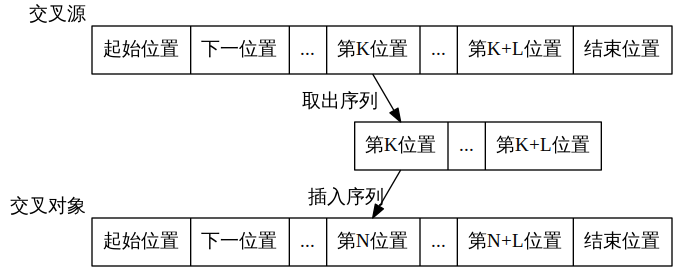
\includegraphics[width=10cm]{pic/life_cross.png}
			\caption{交叉算子}
			\label{fig:cross}
		\end{figure}
		\begin{figure}[htbp]
			\centering
			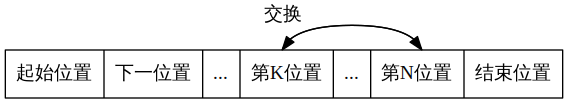
\includegraphics[width=9cm]{pic/life_muate.png}
			\caption{变异算子}
			\label{fig:muate}
		\end{figure}
      %\subsubsection{迭代计算}
        使用上述算法结构对于本问题所给的数据进行种群演化,经过长时间算法运行,得到结果如图\ref{fig:ga},总长度为$2775.273329$
        \begin{figure}[!htbp]
        	\centering
        	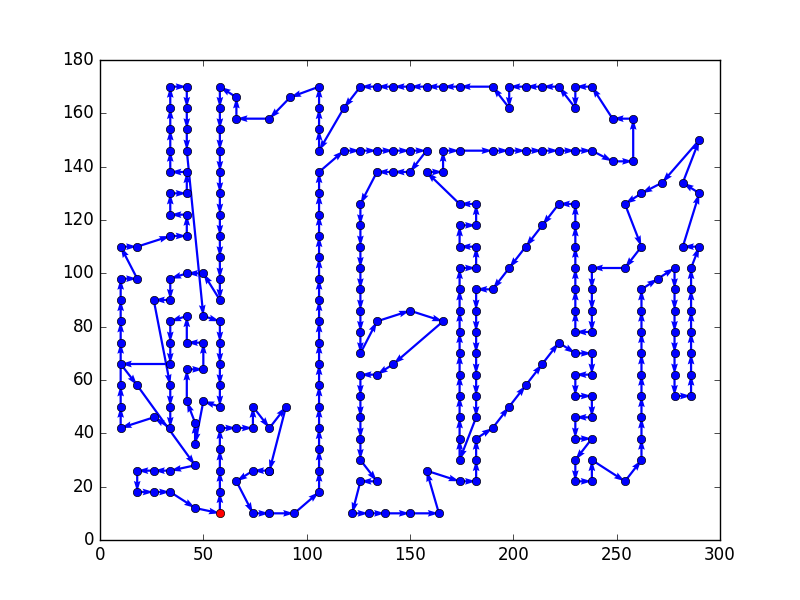
\includegraphics[width=10cm]{pic/ga_result.png}
        	\caption{遗传算法结果}
        	\label{fig:ga}
        \end{figure}
      \subsubsection{改进贪婪算法\cite{饶卫振2012基于求解}}
        贪婪算法是一种构建型启发式算法,其原理是
        求出任意两位点间欧式距离,建立图G的邻接矩阵$D$并为其赋值,其中$d_{i,j}$表示位点$x_i$与$x_j$间的距离。将距离矩
        阵中两位点间距离按从小到大的顺序排列,从最短边开始向图$G$中添加,直至添加到图$G$成为一条回路为止。
        在添加过程中算法遵循以下原则:
        \begin{enumerate}
        	\item 该节点的链接边数小于2。
        	\item 链接的边不会形成边数小于$n$的回路。
        \end{enumerate}
        
         但贪婪算法在寻找过程中并没有主动使起点与终点回合,所以会造成最后返回路径非常长,如图\ref{fig:fail}所示,这时所得到的总长度为$2861.03928238$。
         \begin{figure}[htbp]
            \centering
            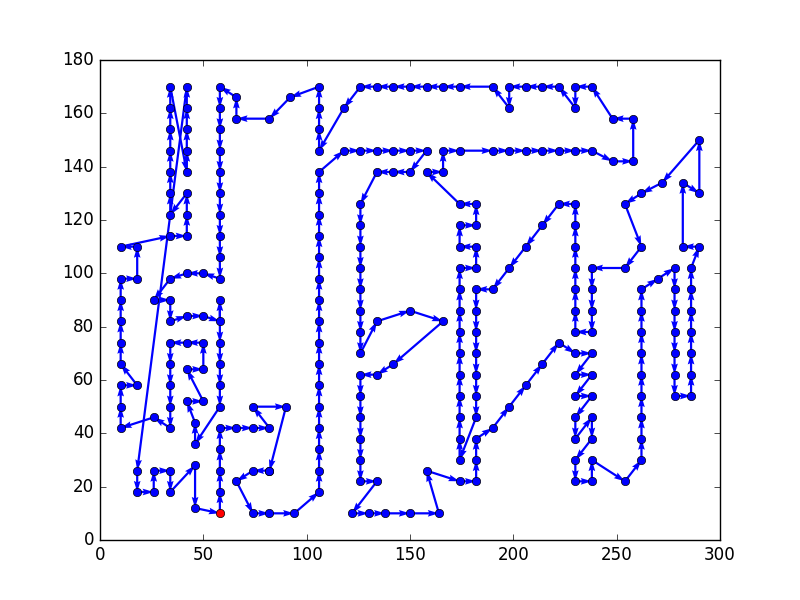
\includegraphics[width=10cm]{pic/greedy_fail.png}
            \caption{贪婪算法得到的结果}
            \label{fig:fail}
        \end{figure}
        
        分析贪婪算法过程可知,算法最后产生的跨度主要由于算法本身没有确定边的拼接方向,依照这种思路对贪婪算法进行改进。
        根据Held与Karp提出的Held-Karp模型\cite{held1970traveling},我们使用一个向量$\pi=(\pi_1,\pi_2,\dots,\pi_k)$对
        贪婪算法的距离矩阵$D$进行改造,如式\ref{equ:held-karp}。
        \begin{equation}
	        D'=\left\{
		        \begin{array}{ll}
		        	d_{i,j} = d_{i,j} - \pi_i - \pi_j & \textrm{$i \neq $j}\\
		        	d_{i,j} = M & \textrm{$i=$j}
		        \end{array}
	        \right.
	        \label{equ:held-karp}
        \end{equation}
        
        其中$M$为一个足够大的数,$\pi_k$由式\ref{equ:pi}构造,其中$\alpha$为比例系数,比例系数越大算法就越倾向于先添加外围的点。
        \begin{equation}
             \left\{
	             \begin{array}{l}
		             \pi=(\pi_1,\pi_2,\dots{,\pi_k}),\pi_k=\alpha\cdot(len_k-\overline{len})\\
		             len_k = \sqrt{(x_0-x_k)^2+(y_0-y_k)^2}\\
		             \overline{len} = \frac{\sum_{k=0}^{k=n}len_k}{n}\\
		             x_0 = \frac{\sum_{k=0}^{k=n}x_k}{n},y_0 = \frac{\sum_{k=0}^{k=n}y_k}{n}
	             \end{array}
             \right.
             \label{equ:pi}
        \end{equation}
 
        根据改进贪婪算法得到最终结果如图\ref{fig:greedy}所示,总长度为$2791.27883397$。
		\begin{figure}[htbp]
			\centering
			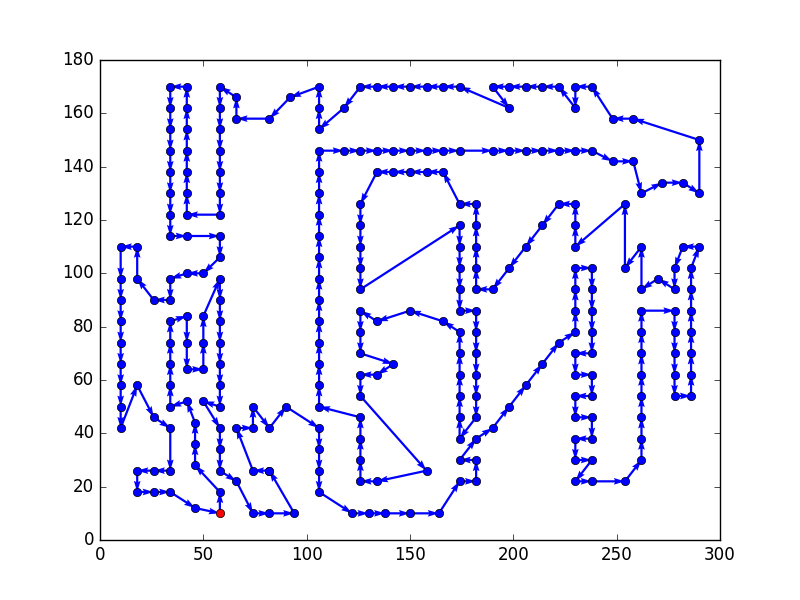
\includegraphics[width=10cm]{pic/greedy_result.png}
			\caption{改进贪婪算法得到的结果}
			\label{fig:greedy}
		\end{figure}

    \subsection{问题二}
      \subsubsection{贪婪算法}
        遗传算法可以获得问题的满意解但是其运行过程十分漫长不适用于题目要求,所以我们
        利用贪婪算法设计了一个较快获得满意解的算法。
      \subsubsection{原理}
        
  \bibliography{mybib}
  \bibliographystyle{gbt7714}
\end{document}
